\documentclass[tikz,border=5pt]{standalone}
\usepackage[utf8]{inputenc}
\usepackage[T1]{fontenc}
\usepackage{lmodern,amsmath,amssymb}
\usepackage[american]{circuitikz}
\usepackage{pgfplots}
\pgfplotsset{compat=1.18}
\usetikzlibrary{circuits.logic.US,positioning,calc,arrows.meta,patterns,shapes.geometric}
\definecolor{Primary}{HTML}{1F77B4}
\begin{document}
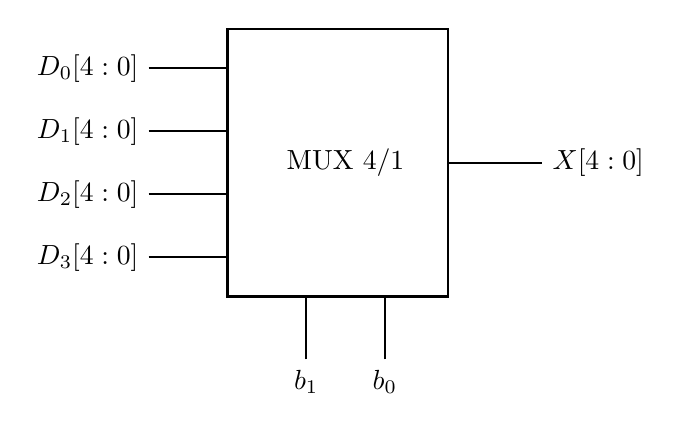
\begin{tikzpicture}[thick]
\draw(0,0)rectangle(2.8,3.4);\node at(1.5,1.7){MUX 4/1};
\foreach \i in {0,1,2,3}{\pgfmathsetmacro{\y}{2.9-.8*\i}\draw(-1,\y)node[left]{$D_\i[4:0]$}--(0,\y);}
\draw(2.8,1.7)--(4,1.7)node[right]{$X[4:0]$};\draw(1,-.8)node[below]{$b_1$}--(1,0);\draw(2,-.8)node[below]{$b_0$}--(2,0);
\end{tikzpicture}
\end{document}
